\section{Introduction}


    \setlength{\intextsep}{0pt}
    \begin{wrapfigure}{r}{\textwidth/2}
        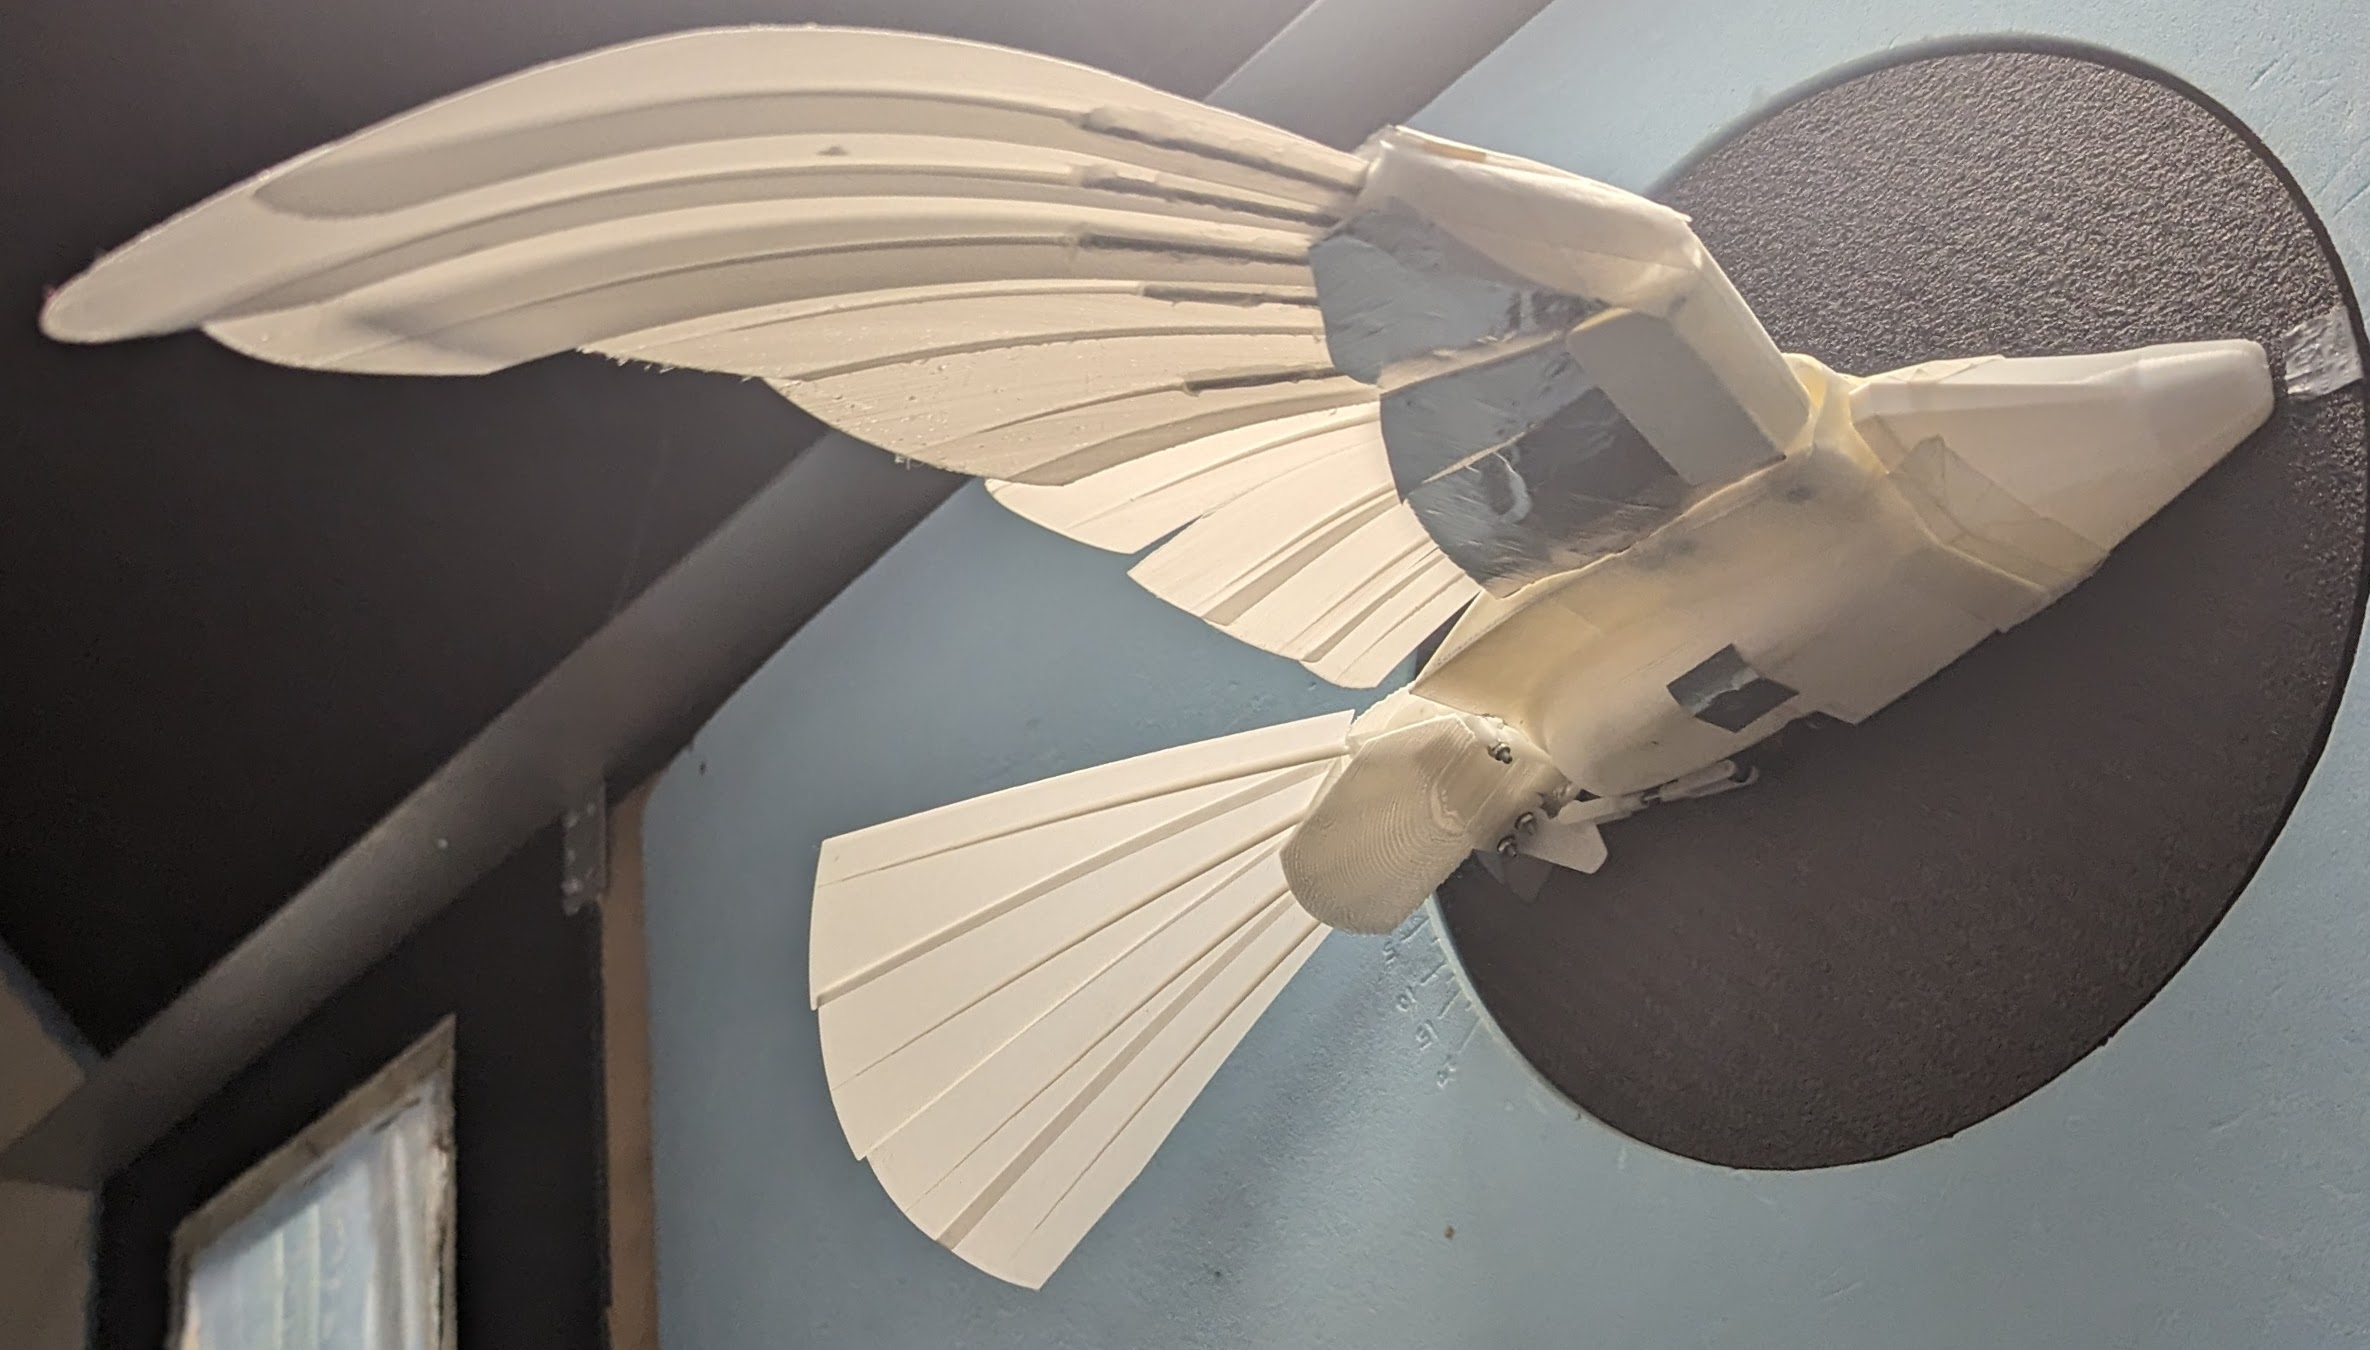
\includegraphics[width=\textwidth/2]{./Resources/Kestrel.jpg}
    \end{wrapfigure}

    Mapping and surveying, environmental monitoring, delivery, search and
    rescue are some of the current applications of Unmanned Arial Vehicles
    (UAVs). Improving their ability to adjust to changes in wind conditions
    is a topic of much research [1] especially as work continues to
    allow UAVs to carry out increasingly complicated tasks autonomously
    like CSIRO’s Hovermap an arial 3D mapping platform [2].
    \vspace{\baselineskip}
    In Australia the height limit to operate a UAV is 120m above ground
    level [3]. At these heights wind turbulence and gust conditions greatly
    impact the performance of UAVs, by changing its trajectory and expected
    current state potentially leading to drone damage. As a response to
    this, researchers have turned to nature as inspiration. Basing UAV
    design on birds has advantages over classical UAV designs (like
    multi-rotor or fixed wing drones) including increased aerodynamic
    efficiency, high manoeuvrability and stability in high-gust conditions
    [4].
    \vspace{\baselineskip}
    In this project we build on existing work to develop stable flight
    controllers for a novel platform the Kestrel robotic replica half-wing
    based on the Nankeen Kestrel with three degrees of freedom (wing
    extension, tail spread and tail pitch) [5]
    (Figure 1).
    As a novel design
    the wing cannot be controlled with existing software, prior work on the
    Kestrel half-wing focussed on utilising Deep Reinforcement Learning
    (DRL) to develop a flight stability controller. DRL has been shown
    to have superior response time, reduced error and ability to reject
    external disturbances. Additionally, development of a DRL controller
    does not require domain specific knowledge in controller tuning [6].
    \vspace{\baselineskip}
    We will investigate the use of a classical controllers on the novel
    Kestrel platform to directly compare it to the DRL controller.
    We aim develop a Proportional Integral Derivative (PID) controller
    for flight stability already shown to be effective in stabilising UAVs
    [7].
    \vspace{\baselineskip}

    \section{Related Work}
    \section{Methodology}
    \section{Results}
    \section{Evaluation}
    \section{Discussion}
    \section{Conclusion}
    \section{References}
